\chapter{DeepSeek}
\section{Multi-Head Latent Attention}

\begin{figure}[h]
	\centering
	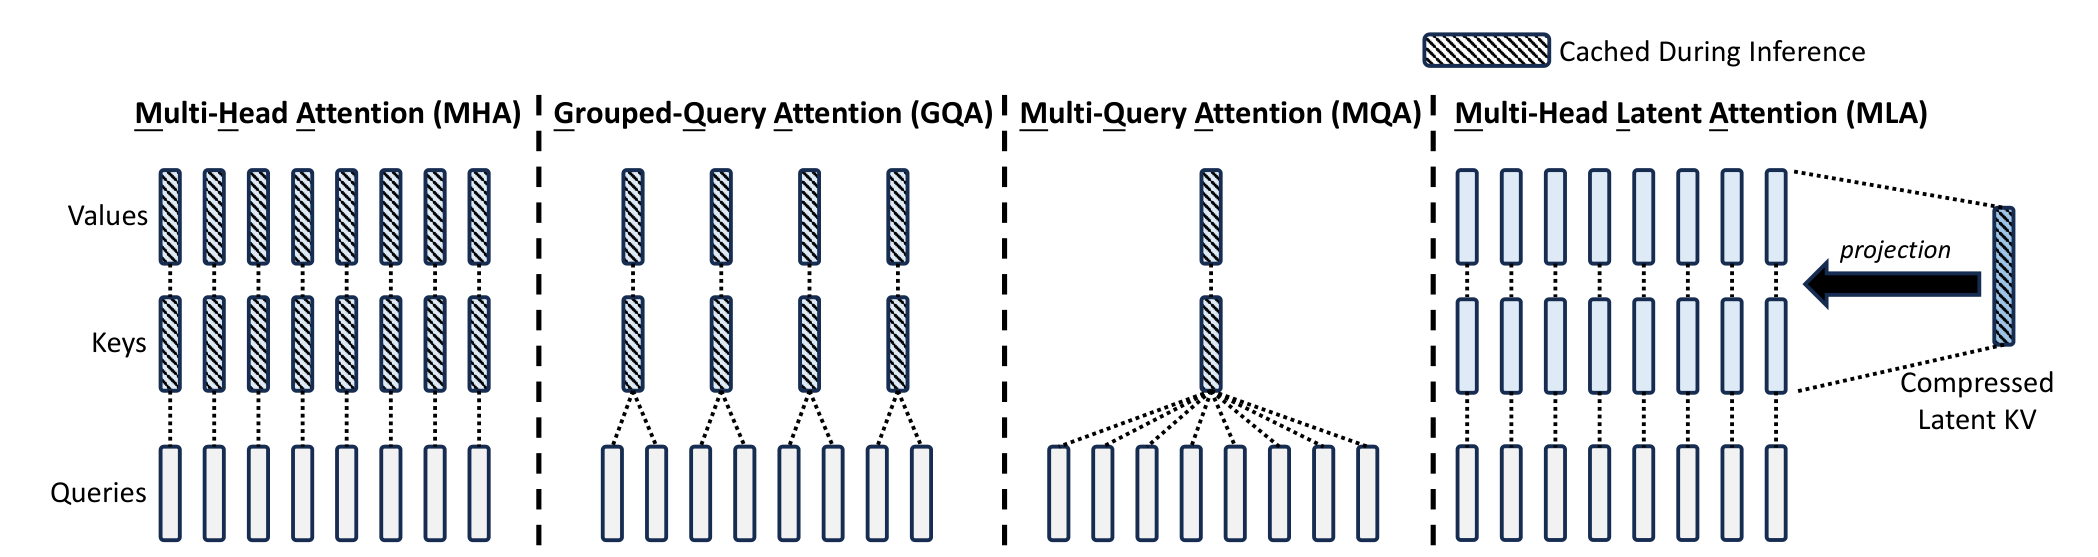
\includegraphics[scale=0.32]{./images/transformer/mla.png}
\end{figure}

The query, key, and value of the vanilla multi-head attention can be expressed as follows:
\begin{align*}
	\rvq_t &= W^{Q}\rvh_t\\
	\rvk_t &= W^{K}\rvh_t\\
	\rvv_t &= W^{V}\rvh_t
\end{align*}
\begin{itemize}
	\item $\rvq_t,\rvk_t,\rvv_t\in \mathbb{R}^{d_hn_h}$
	\item $\rvh_t\in \mathbb{R}^{d}$: Attention input of the $t$-th token at an layer.
	\item $d_h$: the attention head's dimension
	\item $n_h$: the number of attention heads
\end{itemize}

The core of Multi-Head Latent Attention (MLA) is the low-rank joint compression for attention keys and values to reduce Key-Value (KV) cache during inference:
\begin{align*}
	\rvc_t^{KV} &= W^{DKV}\rvh_t\\
	[\rvk_{t,1}^C; \rvk_{t,2}^C; \dots ;\rvk_{t,n_h}^C;] = \rvk_t^{C} &= W^{UK}\rvc_t^{KV}\\
	[\rvv_{t,1}^C; \rvv_{t,2}^C; \dots ;\rvv_{t,n_h}^C;] = \rvv_t^{C} &= W^{UV}\rvc_t^{KV}
\end{align*}
\begin{itemize}
	\item $\rvc_t^{KV}\in \mathbb{R}^{d_c}$ is the compressed \textit{latent vector} for keys and values, where $d_c\ll d_hn_h$. \textbf{Note that this is not a query vector.}
	\item $W^{DKV}\in \mathbb{R}^{d_c\times d}$ is the down-projection matrix
	\item $W^{UK},W^{UV}\in \mathbb{R}^{d_hn_h\times d_c}$ are the up-projection matrices for keys and values, respectively.
	\item During inference, MLA only needs to cache $\rvc_t^{KV}$
	\item Thus, KV cache has only $d_c\times l$ elements, where $l$ is the number of layers.
\end{itemize}
Unlike the MHA, MLA only needs to keep the $\rvc_t^{KV}$ (\ie cache), since we can create the key and the value from the latent vector $\rvc_t$. This leads to a significant memory usage.

Moreover, in order to reduce the activation memory during training, we also perform low-rank compression for the queries, even if it cannot reduce the KV cache:
\begin{align*}
	\rvc_t^{Q} &= W^{DQ}\rvh_t\\
	[\rvq_{t,1}^R; \rvq_{t,2}^R; \dots ;\rvq_{t,n_h}^R;] = \rvq_t^{C} &= W^{UQ}\rvc_t^{Q}
\end{align*}
\begin{itemize}
	\item $\rvc_t^{Q}\in \mathbb{R}^{d_c'}$ is the compressed latent vector for queries, where $d_c'\ll d_hn_h$
	\item $W^{DQ}\in \mathbb{R}^{d_c'\times d}$ and $W^{UQ}\in \mathbb{R}^{d_hn_h\times d_c'}$ are the down- and up- projection matrices for queries, respectively.
\end{itemize}

\section{DeepSeek MoE}

\begin{align*}
	\rvh_t' = \rvu_t+\sum^{N_s}_{i=1}FFN_i^{(s)}(\rvu_t)+\sum^{N_r}_{i=1}g_{i,t}FFN_i^{(r)}(\rvu_t),
\end{align*}
\begin{itemize}
	\item 
		$$g_{i,t} = \frac{g_{i,t}'}{\sum^{N_r}_{j=1}g_{j,t}'}$$
	\item 
		\begin{align*}
			g_{i,t}' = \begin{cases}
				s_{i,t}&\text{ } s_{i,t}\in TopK(\{s_{j,t}|1\leq j \leq N_r\}, K_r)\\
				0&\text{otherwise,}
			\end{cases}
		\end{align*}
	\item 
		$$s_{i,t} = \sigma(\rvu_t^T\rve_i)$$
	\item $\rvu_t$: FFN input of the $t$-th token. 
	\item $\rvh_t'$ FFN output
	\item $N_s$ and $N_r$ are the number of \textit{shared} experts and the \textit{routed} experts, respectively.
	\item $FFN_i^{(s)}(\cdot)$ and $FFN_i^{(r)}(\cdot)$ are the $i$-th \textit{shared} expert and the $i$-th \textit{routed} expert, respectively.
	\item $K_r$ is the number of activated routed experts
	\item $g_{i,t}$: gating value for the $i$-th expert
	\item $s_{i,t}$: a token assigned to an expert (\ie affinity score)
	\item $\rve_i$: the centroid vector of the $i$-th routed expert
	\item $TopK(\cdot, K)$: the set comprising $K$ highest scores among the affinity scores calculated for the $t$-th token and all routed experts.
	\item $\sigma$: Sigmoid function.
\end{itemize}

Let's closely look at the equation
\begin{align*}
	\rvh_t' = \rvu_t+\sum^{N_s}_{i=1}FFN_i^{(s)}(\rvu_t)+\sum^{N_r}_{i=1}g_{i,t}FFN_i^{(r)}(\rvu_t),
\end{align*}
\begin{itemize}
	\item $\rvu_t+\dots$: this is just a skip connection
	\item $\sum^{N_s}_{i=1}FFN_i^{(s)}(\rvu_t)$: Always activated
	\item $\sum^{N_r}_{i=1}g_{i,t}FFN_i^{(r)}(\rvu_t)$
\end{itemize}



